%% Chapter 3: Experimental Setup / Methodology (chapters/chapter03.tex)

% ==============================================================================
% Chapter Writing Guidelines:
% - Materials: Specify the list of equipment, components, and substances used.
% - Methodology: Outline step-by-step procedures.
% - Diagram: Provide a clear block diagram or optical schematic.
% - Code snippets: Document details of data acquisition/analysis scripts.
% ==============================================================================

\chapter{Experimental Setup and Methodology}
\label{ch:methodology}

This chapter details the experimental setup designed for Z-scan measurements and lists the Python simulation script used to analyze the intensity profile.

\section{Z-Scan Setup Block Diagram}
Figure \ref{fig:zscan_block} shows the signal flow diagram of our measurement configuration.

\begin{figure}[H]
    \centering
    \begin{tikzpicture}[
        node distance=2.5cm,
        block/.style={draw, rectangle, fill=blue!10, minimum width=2.5cm, minimum height=1cm, align=center, rounded corners},
        arrow/.style={-Latex, thick}
    ]
        % Nodes
        \node (laser) [block] {He-Ne Laser\\($\lambda = 632.8$ nm)};
        \node (lens) [block, right of=laser, node distance=3.5cm] {Focusing Lens\\($f = 100$ mm)};
        \node (sample) [block, right of=lens, node distance=3.5cm] {Sample Stage\\(Motorized)};
        \node (detector) [block, right of=sample, node distance=3.5cm] {Photodetector\\(Silicon)};
        \node (daq) [block, below of=sample, node distance=2.0cm] {DAQ / PC\\(Data Analysis)};

        % Paths
        \draw [arrow] (laser) -- (lens);
        \draw [arrow] (lens) -- (sample);
        \draw [arrow] (sample) -- (detector);
        \draw [arrow] (detector) |- (daq);
        \draw [arrow] (daq) -- (sample) node[midway, left] {Control};
    \end{tikzpicture}
    \caption{Signal flow block diagram of the Z-scan experimental system.}
    \label{fig:zscan_block}
\end{figure}

\section{Optical Table Layout Schematic}
Using TikZ and custom node shapes, we represent the optical layout schematic below:

\begin{figure}[H]
    \centering
    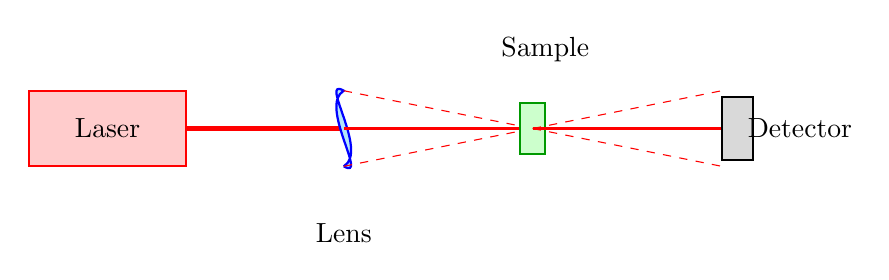
\begin{tikzpicture}[scale=0.8]
        % Laser source
        \draw[fill=red!20, draw=red, thick] (0, 0) rectangle (2.5, 1.2) node[midway] {Laser};
        \draw[red, line width=1.5pt] (2.5, 0.6) -- (5.0, 0.6); % beam before lens
        
        % Lens representation
        \draw[fill=cyan!30, draw=blue, thick] (5.0, 0) to[out=30, in=150] (5.0, 1.2) to[out=-150, in=-30] (5.0, 0) node[below=0.6cm] {Lens};
        
        % Focused beam converging to focal point
        \draw[red, line width=1.0pt] (5.0, 0.6) -- (8.0, 0.6);
        \draw[red, dashed] (5.0, 1.2) -- (8.0, 0.6);
        \draw[red, dashed] (5.0, 0) -- (8.0, 0.6);
        
        % Sample at focal point
        \draw[fill=green!20, draw=green!60!black, thick] (7.8, 0.2) rectangle (8.2, 1.0) node[above=0.4cm] {Sample};
        
        % Diverging beam after focal point
        \draw[red, dashed] (8.0, 0.6) -- (11.0, 1.2);
        \draw[red, dashed] (8.0, 0.6) -- (11.0, 0);
        \draw[red, line width=1.0pt] (8.0, 0.6) -- (11.0, 0.6);
        
        % Detector
        \draw[fill=gray!30, draw=black, thick] (11.0, 0.1) rectangle (11.5, 1.1) node[midway, right] {Detector};
    \end{tikzpicture}
    \caption{Schematic representation of the single-lens closed-aperture Z-scan configuration.}
    \label{fig:optical_schematic}
\end{figure}

\section{Circuit Diagram Example}
An example electronics circuit configuration for the detector amplification stage using \textsf{circuitikz} is shown in Figure \ref{fig:amplifier_circuit}:

\begin{figure}[H]
    \centering
    \begin{circuitikz}[scale=0.8]
        \draw (0,0) node[op amp] (opamp) {}
        (opamp.-) -- (-1.5,0.5) to[R, l=$R_1$] (-3,0.5) node[ground] {}
        (opamp.+) -- (-1.5,-0.5) to[empty photodiode, l=$D_{in}$] (-3,-0.5) node[ground] {}
        (opamp.-) -- (-1.5,0.5) -- (-1.5,2) to[R, l=$R_f$] (1.5,2) -| (opamp.out)
        (opamp.out) -- (1.5,0) node[right] {$V_{out}$};
    \end{circuitikz}
    \caption{Photodiode transimpedance amplifier schematic circuit diagram.}
    \label{fig:amplifier_circuit}
\end{figure}

\section{Analysis Code Script}
We use the following Python script to calculate the normalized transmission profile:
\begin{lstlisting}[style=pythonstyle, caption={Python routine for processing closed-aperture Z-scan values.}, label={lst:zscan_python}]
import numpy as np

def calculate_transmission(z, delta_phi):
    """
    Calculates normalized transmission for a third-order
    non-linear refractive index change.
    """
    x = z / 1.0 # normalized z coordinate
    transmission = 1 + (4 * delta_phi * x) / ((x**2 + 9) * (x**2 + 1))
    return transmission

# Sample coordinate generation
z_values = np.linspace(-5, 5, 100)
trans = calculate_transmission(z_values, delta_phi=0.5)
print("Peak transmission calculated at normalized position.")
\end{lstlisting}
